\section{\Tikz}
  Libreria grafica per disegnare (descrivere disegni) con LaTeX.\\
  Offre un piano cartesiano su cui disegnare mediante dei comandi.\\~\\
  \texttt{\textbackslash{}usepackage\{tikz\} \%preambolo}\\
  \dots\\\texttt{
  \textbackslash{}begin\{tikzpicture\}\\
  \dots\\
  \textbackslash{}end\{tikzpicture\}~~\\~}
\subsection{Disegnare}
\subsubsection{Punti}
  \texttt{(1cm,2pt)} è un punto a coordinata x 1cm dall'origne e y 2pt dall'origine\\~\\
  \texttt{(30:1cm)} è un punto sulla circonferenza di raggio 1 cm, a 30 gradi (coordinate polari)\\~\\
  \texttt{++(1cm,2cm)} le coordinate sono relative a quelle del punto precedente e non all'origine\\~\\
  \texttt{+(1cm,2cm)} come \texttt{++} ma non aggiorna le coordinate dell'ultimo punto
\subsubsection{path}
  \texttt{\textbackslash{}path[opzioni] punti;}\\
  \begin{description}
    \item[path type] \texttt{\textbackslash{}draw}, \texttt{\textbackslash{}fill}, \texttt{\textbackslash{}filldraw}
    \item[geometria] \texttt{rotate=<angolo>}, \texttt{xshift=<length>}, \texttt{yshift}, \texttt{scale=<fattore>}
    \item[colore] \texttt{color=<colore>}, \texttt{draw=<colore>}, \texttt{fill=<colore>}, \texttt{opacity=<fattore>}
    \item[spessore linee] ultra thin, very thin, thin, semithick, thick, very thick, ultra thick
    \item[tratteggio] solid, dashed, dotted, dashdotted, densely dotted, loosely dotted, "double
  \end{description}
\subsubsection{Esempi}
  \begin{tabular}{l|l}
    \texttt{\small\textbackslash{}draw (1,0) -\hspace{0.01mm}- (0,0) -\hspace{0.01mm}- (0,1);} & \begin{tikzpicture}\draw (1,0) -- (0,0) -- (0,1);\end{tikzpicture}\\\hline~&~\\
    \texttt{\small\textbackslash{}draw[red, dashed, very thick, rotate=30] (1,0) -\hspace{0.01mm}- (0,0) -\hspace{0.01mm}- (0,1);} & 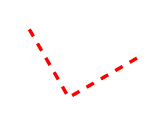
\begin{tikzpicture}\draw[red, dashed, very thick, rotate=30] (1,0) -- (0,0) -- (0,1);\end{tikzpicture} \\\hline~&~\\
    \texttt{\small\textbackslash{}fill (1,0) -\hspace{0.01mm}- (0,0) -\hspace{0.01mm}- (0,1) -\hspace{0.01mm}- cycle;} & 
\begin{tikzpicture}\fill (1,0) -- (0,0) -- (0,1) -- cycle;\end{tikzpicture}\\\hline~&~\\
    \texttt{\small\textbackslash{}draw (0,0) -| (0.5,1) (1,0) |- (2,1);} & \begin{tikzpicture}\draw (0,0) -| (0.5,1) (1,0) |- (2,1);\end{tikzpicture}
  \end{tabular}
\subsubsection{Figure geometriche}
  \begin{tabular}{l|l}
    \texttt{\small\textbackslash{}draw (0,0) rectangle (2,1);} & 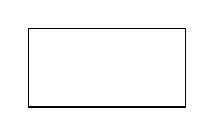
\begin{tikzpicture}\draw (0,0) rectangle (2,1);\end{tikzpicture}\\\hline~&~\\
    \texttt{\small\textbackslash{}draw (0,0) circle [radius=1];} & 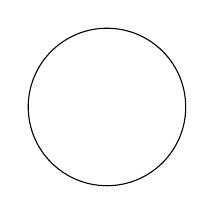
\begin{tikzpicture}\draw (0,0) circle [radius=1];\end{tikzpicture} \\\hline~&~\\
    \texttt{\small\textbackslash{}draw  (0,0) circle [x radius=1cm, y radius=5mm, rotate=30];} & 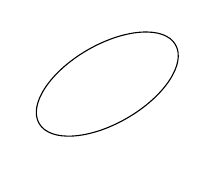
\begin{tikzpicture}\draw  (0,0) circle [x radius=1cm, y radius=5mm, rotate=30];\end{tikzpicture}\\
  \end{tabular}
\subsubsection{Nodi}
  \begin{tabular}{l|l}\texttt{\small\textbackslash{}draw (0,0) node \{centro\} circle [radius=1];} & 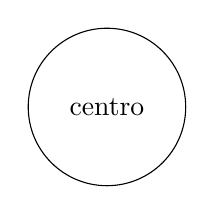
\begin{tikzpicture}\draw (0,0) node {centro} circle [radius=1];\end{tikzpicture} \\\hline\\
    \begin{tabular}{l}\texttt{\small\textbackslash{}draw (0,0) node (centro) \{O\} circle [radius=5mm];}\\\texttt{\small\textbackslash{}draw (centro) rectangle ++(1,1);}\end{tabular} & 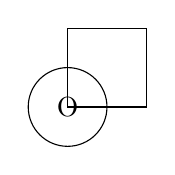
\begin{tikzpicture}\draw  (0,0) node (centro) {O} circle [radius=5mm];\draw (centro) rectangle ++(1,1);\end{tikzpicture}\\
  \end{tabular}

\subsection{Grafici}
  {\[g(x)=e^x;~~h(x)=x^2;~~i(x)=x-3; \]\[f(x)=\begin{cases}  g(x) & x<-1\\
                        h(x) & -1<x<2\\
                        i(x) & x>2
          \end{cases}\]}
  {\centering
    \begin{tikzpicture}
      \draw[->] (-6,0) -- (6,0) node[below] {$x$};
          \draw[->] (0,-2) -- (0,5) node[left] {$y$};
          \draw[loosely dotted] (-5.9,-1.9) grid (5.9,4.9);
          %1-s(x+1)
          \draw[domain=-1:6,thick,variable=\x,red] plot ({\x},{0});
          \draw[domain=-6:-1,smooth,variable=\x,red] plot ({\x},{1});
          %s(x+1)[1-s(x-2)]
          \draw[domain=2:6,smooth,dashed,variable=\x,green] plot ({\x},{0});
          \draw[domain=-6:-1,smooth,variable=\x,green] plot ({\x},{0});
          \draw[domain=-1:2,smooth,variable=\x,green] plot ({\x},{1});
          %s(x-2)
          \draw[domain=-6:2,smooth,dashed,variable=\x,cyan] plot ({\x},{0});
          \draw[domain=2:6,smooth,variable=\x,cyan] plot ({\x},{1});
          %f(x)
          \draw[domain=-6:-1,smooth,variable=\x,blue] plot ({\x},{e^\x});
          \draw[domain=-1:2,smooth,variable=\x,blue] plot ({\x},{\x*\x});
          \draw[domain=2:6,smooth,variable=\x,blue] plot ({\x},{\x-3});
          \draw[smooth,blue,fill=white] (-1,1/e) circle (1.5pt);
          \draw[smooth,black,fill=white] (-1,1) circle (1.5pt);
          \draw[smooth,blue,fill=white] (2,4) circle (1.5pt);
          \draw[smooth,blue,fill=white] (2,-1) circle (1.5pt);
          \draw[smooth,black,fill=white] (-1,0) circle (1.5pt);
          \draw[smooth,black,fill=white] (2,0) circle (1.5pt);
          \draw[smooth,black,fill=white] (2,1) circle (1.5pt);
    \end{tikzpicture}\par
  }
  {\[\color{blue}y=f(x)=\frac{1}{2}[e^x+(x+1)^{l-1}(x^2-e^x)-(x-2)^{l-1}(x^2-x+3)+x-3]\]
  \[{\color{red}y=\se{-\infty}{-1}(x)=\1(-x-1)}~~{\color{green}y=\se{-1}{2}(x)}~~{\color{cyan}y=\se{2}{\infty}(x)=\1(x-2)}\]}
\subsubsection{Grafici con \Tikz}
  \begin{flushleft}
    \texttt{~\\
    \textbackslash{}begin\{tikzpicture\}\\
    ~~\%assi cartesiani\\
    ~~\textbackslash{}draw[-\textgreater{}] (-9,0) -\hspace{0.01mm}- (9,0) node[below] \{\textdollar{}x\textdollar{}\};
\\
    ~~\textbackslash{}draw[-\textgreater{}] (0,-1.3) -\hspace{0.01mm}- (0,4.2) node[left] \{\textdollar{}y\textdollar{}\};\\
    ~~\%griglia\\
    ~~\textbackslash{}draw[loosely dotted] (-8.9,-1.2) grid (8.9,4.2);\\
    ~~\%funzione
\\
    ~~\textbackslash{}draw[domain=-1:8.9,thick,red] plot (\{\textbackslash{}x\},\{\textbackslash{}x\^{}2\});
\\
    \textbackslash{}end\{tikzpicture\}\\~
    }
    \end{flushleft}
\subsubsection{Funzioni}
 factorial(x), sqrt(x), pow(x,y), exp(x), ln(x), log10(x), log2(x), abs(x), mod(x,y), round(x), floor(x), ceil(x), sin(x), cos(x), tan(x), min(x,y,) e max(x,y).\\~\\
 Gli argomenti delle funzioni trigonometriche vanno espressi in gradi; per esprimerli in radianti bisogna postporre una \emph{r}.\\~\\
 Si possono usare le costanti: \texttt{e} e \texttt{pi}.

\subsection{Mappe Concettuali}
  \texttt{\textbackslash{}usetikzlibrary\{mindmap\}}\\
        \texttt{\textbackslash{}begin\{tikzpicture\}[mindmap, concept color=yellow]\\
~~\textbackslash{}node [concept] \{Parola chiave\}\\
~~~~child[grow=0] \{\\
~~~~~~node[concept] \{figlio 1\}\\
~~~~~~child[concept color=green] \{node[concept] (nipote) \{nipote\}\}\\
~~~~\}\\
~~~~child[concept color=orange,grow=30] \{node[concept] (figlio) \{figlio 2\}\};\\
~~\textbackslash{}draw [concept connection]  (figlio) edge (nipote);
}\\

      \begin{tikzpicture}[mindmap, concept color=yellow]
        \node [concept] {Parola\\chiave}
          child[grow=0] {
            node[concept] {figlio 1}
            child[concept color=green] {node[concept] (nipote) {nipote}}
          }
          child[concept color=orange,grow=30] {node[concept] (figlio) {figlio 2}};
          \draw [concept connection]  (figlio) edge (nipote);
      \end{tikzpicture}

